
\documentclass{beamer}

% http://deic.uab.es/~iblanes/beamer_gallery/index_by_theme.html
\mode<presentation>
{
  \usetheme{Madrid}       % or try default, Darmstadt, Warsaw, ...
  \usecolortheme{default} % or try albatross, beaver, crane, ...
  \usefonttheme{serif}    % or try default, structurebold, ...
  \setbeamertemplate{navigation symbols}{}
  \setbeamertemplate{caption}[numbered]
} 


%%% standard packages %%%
\usepackage[english]{babel}
\usepackage[utf8x]{inputenc}
\usepackage{chemfig}
\usepackage[version=3]{mhchem}

%%% documentation %%%
\usepackage{hyperref}
\usepackage{natbib}
\bibliographystyle{agsm}

%%% spacing, fonts, etc %%%
\usepackage{setspace}
\usepackage{amsfonts} 

%%% animate! %%%
\usepackage{animate}
\usepackage{xmpmulti}


\title[Trend Segmentation]{Uses of High Dimensional Trend Segmentation}
\institute[LSE Department of Statistics]{}

\bigskip

\author[]{
\\
  {Shakeel Gavioli-Akilagun} \\
  \footnotesize{Supervisor: Prof. Piotr Fryzlewicz}
}

\date[02 June 2020]{
  \hspace{1cm}\\
  PhD Presentation Event\\
  \hspace{1cm}\\
  {\fontfamily{pcr}\selectfont \href{https://github.com/Shakeel95/PhD-Presentation-1}{$\left \{ \text{code} \right \}$}}
}

\setcounter{tocdepth}{1}

\begin{document}



%%% Title Page %%% 

\begin{frame}
  \titlepage
\end{frame}



%%% Table of contents %%%

\begin{frame}{Roadmap}
  \tableofcontents
\end{frame}



%%%%%%%%%%%%%%%%%%%%%%%%%%%
%% SECTION 1: Motivation %%
%%%%%%%%%%%%%%%%%%%%%%%%%%%

\section{Motivation}



%%% Table of contents %%%

\begin{frame}{Roadmap}
\tableofcontents[currentsection]
\end{frame}



%%% SS %%%
\subsection{motivation for trend segmentation}



%%% Present motivating data example %%%

\begin{frame}{Motivation for Trend Segmentation}
\framesubtitle{S\&P 500 around COVID-19 outbreak}

Opening prices and log-returns for all S\&P 500 constituents around the COVID-19 outbreak. It may be of interest to find groups of time series which responded similarly to the shock.

\begin{figure}[H]
    \centering
    \begin{subfigure}
        \includegraphics[width = 0.45\textwidth]{../plots/SnP500_raw_COVID.png}
    \end{subfigure}
    \begin{subfigure}
        \includegraphics[width = 0.45\textwidth]{../plots/SnP500_LR_COVID.png}
    \end{subfigure}
\end{figure}

\end{frame}



%%% SnP Correlation Clustering %%%

\begin{frame}{Motivation for Trend Segmentation}
\framesubtitle{Clustering on instantaneous correlation of log-returns}

A common first step in EDA. Transform time series to stationarity $x_t \equiv \Delta \log \left ( X_t \right )$, then measure distance as $d(X,Y) = 1-\left | \text{cor} \left ( x,y \right ) \right |$.

\begin{figure}
    \centering
    \onslide<2->{\begin{subfigure}
        \includegraphics[width = 0.3\textwidth]{../plots/SnP500_cor_similar.png}
    \end{subfigure}}
        \onslide<3->{\begin{subfigure}
        \includegraphics[width = 0.3\textwidth]{../plots/SnP500_random_selection.png}
    \end{subfigure}}
        \onslide<4->{\begin{subfigure}
        \includegraphics[width = 0.3\textwidth]{../plots/SnP500_cor_dissimilar.png}}
    \end{subfigure}
\end{figure}
    
\end{frame}



%%% Model based clustering %%%

\begin{frame}{Motivation for Trend Segmentation}
\framesubtitle{Model based clustering}

% $l_2$-distance between models introduced by \cite{piccolo1990distance} and generalised by \cite{otranto2004classifying}.

Let $x_t \sim \text{GARCH}(p,q)$, under invertibility
$x_t^2 = \sum_{i=1}^\infty \pi_{i} x_{t-i}^2 + \eta_{t}$. Measure distance as: $ d\left ( X, Y \right ) = \left \{ \sum_{i=1}^\infty \left ( \pi_{x,i} - \pi_{y,i} \right )^2 \right \}^{\frac{1}{2}}$. 

\bigskip

\begin{figure}
    \centering
    \begin{subfigure}
        \includegraphics[width = 0.4\linewidth]{../plots/SnP500_garch_dissimilar_1.png}
    \end{subfigure}
    \begin{subfigure}
        \includegraphics[width = 0.4\linewidth]{../plots/SnP500_garch_dissimilar_2.png}
    \end{subfigure}\
\end{figure}

\end{frame}



%%% Distance between changepoint skeletons %%%

\begin{frame}{Motivation for Trend Segmentation}
\framesubtitle{Distance between ``changepoint skeletons"}

\begin{columns}

    \begin{column}{0.6\textwidth}
    {\small
    A new measure based on changepoints and the Fréchet distance. Estimate the following: (1) underlying signal  $\widehat{f}: [1,T] \rightarrow \mathbb{R}$, and (2) scaled signal: $\widehat{Q}: [0,1] \rightarrow [0,1]$. Then:

    \begin{align*}
        d(X,Y) = \underset{\alpha,\beta}{\inf} \left \{ \underset{t \in [0,1]}{\max} \left \| \widehat{Q}_X\left ( \alpha(t) \right ) - \widehat{Q}_Y\left ( \beta(t) \right ) \right \| \right \}
    \end{align*}
    
    \text{}
    
    Where $\alpha, \beta : [0,1] \rightarrow [0,1]$. Whole dissimilarity matrix can be computed in $\mathcal{O} \left ( n^2T \right )$ time. 
    }
    \end{column}
    
    \begin{column}{0.4\textwidth}
    \begin{figure}
        \centering
        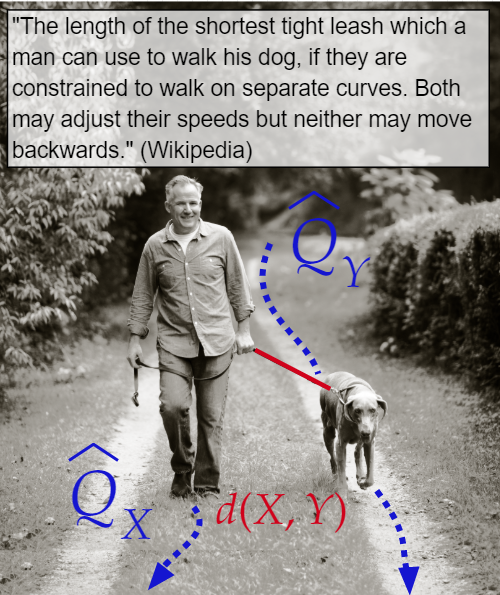
\includegraphics[width = 1\textwidth,left]{../plots/frechet_dist_illustration.jpg}
    \end{figure}
    \end{column}
    
\end{columns}
    
\end{frame}



%%% Changepoint Skeletons: results %%% 

\begin{frame}{Motivation for Trend Segmentation}
\framesubtitle{Distance between ``changepoint skeletons"}

Clusters from the new procedure contain time series with similar behaviour before and after the shock:

\bigskip

\begin{figure}
    \centering
    \begin{subfigure}
        \includegraphics[width = 0.3\textwidth]{../plots/SnP500_frechet_similar_1.png}
    \end{subfigure}
    \begin{subfigure}
        \includegraphics[width = 0.3\textwidth]{../plots/SnP500_frechet_similar_2.png}    
    \end{subfigure}
    \begin{subfigure}
        \includegraphics[width = 0.3\textwidth]{../plots/SnP500_frechet_similar_3.png}
    \end{subfigure}
\end{figure}
    
\end{frame}



%% SS %%
\subsection{Derived Model}



%%% Model Setup %%%

\begin{frame}{Derived Model}
\framesubtitle{Univariate trend segmentation}

Given a sample $\left \{ X_t \right \}_{t=1}^{T}$ assume a `signal + noise' model $X_t = f(t) + \varepsilon_t$ with $\varepsilon_t \sim \left ( 0, \sigma^2 \right )$ and $f(t)$ can be segmented into $N+1$ linear segments with breaks at $0 = \tau_0 < \tau_1 < \dots \tau_N < \tau_{N+1}=T$. Specifically: 

\bigskip

\begin{equation*}
f(t) = 
\left\{\begin{matrix}
        \theta_{1,\tau_1} + t \cdot \theta_{2,\tau_1} & t \in (\tau_0, \tau_1] \\ 
        \theta_{1,\tau_2} + t \cdot \theta_{2,\tau_2} & t \in (\tau_2, \tau_3]\\ 
        \vdots & \\ 
        \theta_{1,\tau_N} + t \cdot \theta_{2,\tau_N} & t \in (\tau_N,\tau_{N+1}]
\end{matrix}\right.
\end{equation*}

\bigskip

Both $N$ and $\left \{ \tau_1, \dots \tau_N \right \}$ are unknown.

\end{frame}



%%% Multivariate trend segmentation %%%

\begin{frame}{Derived Model}
\framesubtitle{Multivariate trend segmentation}

From a sample $\left \{ \boldsymbol{X}_t \right \}_{t=1}^T$ assume a multivariate `signal + noise' model $\boldsymbol{X_t} = \boldsymbol{F}(t) + \boldsymbol{\varepsilon}_t$ with $\boldsymbol{\varepsilon}_t \sim \left ( \boldsymbol{0}, \Sigma \right )$ and $\boldsymbol{F}(t)$ is the concatenation of $n$ piecewise constant function. Specifically: 

\bigskip

\begin{itemize}
    \item $\boldsymbol{X_t} = \left ( X_{1,t},...,X_{n,t}\right )'$
    \item $\boldsymbol{F}(t) = \left ( f_1(t), ..., f_n(t)\right )'$
    \item $\left \{ f_i\right \}_{i=1}^n$ share common changepoints $\left \{ \tau_j \right \} _{j=1}^N$
\end{itemize}

\bigskip

We may have that $T \ll n$. 

\end{frame}




%%% Modelling Objectives %%%

\begin{frame}{Derived Model}
\framesubtitle{Objectives of trend segmentation}

%\doublespacing
The goal is to construct estimates $\left ( \boldsymbol{\widehat{\theta}}, \boldsymbol{\widehat{f}} \right )$ where $\boldsymbol{f} = \left \{ f(t) \right \}_{t=1}^T$ and  $\boldsymbol{\widehat{\theta}} = \left ( \widehat{N}, \widehat{\tau}_1, ..., \widehat{\tau}_{\widehat{N}} \right )$ which allow us to perform one or both of the following tasks with some guarantee of statistical accuracy.

\bigskip

\begin{enumerate}
    \item Changepoint recovery $\mathbb{P} \left ( \widehat{N} = N, \underset{j}{\max} \left | \widhat{\tau_j} - \tau_j \right | \leq g(T) \right ) \rightarrow 1 $
    \item Signal recovery $\mathbb{P} \left ( \left \| \boldsymbol{\widehat{f} - f} \right \|_p \leq g(T) \right ) \rightarrow 1 $
\end{enumerate}

\bigskip

As $T$ (and $n$) $\rightarrow \infty$.

\end{frame}





%%%%%%%%%%%%%%%%%%%%%%%%%%%%%%%%%%%%%%%%%%%%%%%%%%%%%%
%% SECTION 2: Univariate Trend Segmentation Methods %%
%%%%%%%%%%%%%%%%%%%%%%%%%%%%%%%%%%%%%%%%%%%%%%%%%%%%%%

\section{Univariate Trend Segmentation}



%%% Table of contents %%%

\begin{frame}{Roadmap}
\tableofcontents[currentsection]
\end{frame}



%% SS %%
\subsection{Pose discrete optimisation problem}



%%% Comparison with mean-shift methods %%%

\begin{frame}{Mean-Shift Methods Are Not Your Friend!}

\begin{itemize}

    \item Exact search is (NP) hard - \cite{weinmann2015iterative}

    \item Naive approach based on differencing fails even at performing signal recovery - \cite{maidstone2016efficient}
    
    \item Top down approach is inconsistent - \cite{baranowski2019narrowest}
    
\end{itemize}

\end{frame}



%%% Trend segmentation as discrete optimisation %%% 

\begin{frame}{Trend Segmentation as Discrete Optimisation}

Trend segmentation can be posed as a discrete discrete optimisation problem. A solution can be found using exhaustive search - see \cite{tome2004piecewise} and \cite{karl2000record} - but this takes $\mathcal{O}(2^T)$ time!

\begin{align*}
    \boldsymbol{\widehat{\theta}} & = \underset{\boldsymbol{\theta} \in \Theta}{\arg\min} \left \{ \sum_{i=0}^{N-1} \mathcal{C} \left ( \left \{ X_t \right \}_{\tau_i+1}^{\tau_{i+1}}; \boldsymbol{\theta} \right ) + N \cdot \lambda_{(T, \sigma)} \right \} \\
     \onslide<2->{ & \underset{\mathcal{N}}{=} \underset{\boldsymbol{\theta} \in \Theta}{\arg\min} \left \{ \sum_{i=0}^{N-1} \left [ \frac{1}{\sigma^2} \sum_{t = \tau_i + 1}^{\tau_{i+1}}
    \left ( X_t - \left ( \theta_{1, \tau_{i+1}} + t \cdot \theta_{2,\tau_{i+1}} \right ) \right )^2\right ] + N \cdot \lambda_{(T, \sigma)} \right \}}
\end{align*}

\end{frame}



%%% Dynamic programming %%% 

\begin{frame}{Optimisation by Dynamic Programming}
\framesubtitle{Methods for avoiding exhaustive search}
    
\cite{maidstone2017detecting} propose a dynamic programming solution. Let $\mathcal{T}_t$ be set of all possible changepoints on $[1,t]$. Define the cost of optimal segmentation over $[1,t]$ as follows:

\begin{align*}
    h^t(z) & = \underset{\boldsymbol{\tau},k,\left \{z_t \right \}_0^k}{\min} \left \{ \sum_{i=0}^{k-1} \mathcal{C} \left ( \left \{ X_t \right \}_{\tau_i+1}^{\tau_{i+1}}; z_{\tau_i}, z_{\tau_{i+1}} \right ) + ... \\
    & \hspace{2cm} ... + \mathcal{C} \left ( \left \{ X_t \right \}_{\tau_k+1}^{t}; z_{\tau_i}, z_{\tau_{i+1}} \right ) + \lambda \cdot (k+1) \left.  \right \} \\
    \onslide<2->{& = \underset{z',s}{\min} \left \{ h^s(z') + \mathcal{C} \left ( \left \{ X_t \right \}_{s+1}^t; z',z \right ) + \lambda \right \}}
\end{align*}

\onslide<3->{Letting $h^t(z) = \min_{\boldsymbol{\tau} \in \mathcal{T}_t} \left \{ h_{\boldsymbol{\tua}}^t(z) \right \}$, minimising $h^T(z)$ solves the segmentation problem. \underline{Functional pruning}: for $s < t$ if $\boldsymbol{\tau}$ is not optimal over $[1,s]$ then $\left ( \boldsymbol{\tau}, s \right )$ will not be optimal over $[1,t]$.}

\end{frame}



%% SS %%
\subsection{Greedy optimisation}



%%% Greedy optimisation (motivation) %%%

\begin{frame}{Greedy Optimisation}
\framesubtitle{Greedy approximation works well for mean shift problems, does it generalise?}

Greedy solution could be found by recursively applying generalised likelihood ratio test to regions of the signal. For $0<s<b<e\leq T$ let $m \left ( \cdot \right )$ be monotone increasing. Define $\chi_{(s,b,e)} \equiv \chi_{(s,b,e)} \left ( \left \{ x_t \right \}_{s}^e \right )$ as:

\begin{align*}
    \chi_{(s,b,e)} & = m \left ( \left | 
    2\log \left \{ \frac{\underset{\boldsymbol{\theta_1,\theta_2}}{\sup} \hspace{0.2cm} \mathcal{L} \left ( \left \{ X_t \right \}_s^b; \boldsymbol{\theta_1} \right ) \times \mathcal{L} \left ( \left \{ X_t \right \}_{b+1}^e; \boldsymbol{\theta_2} \right )}{\underset{\boldsymbol{\theta}}{\sup} \hspace{0.2cm} \mathcal{L} \left ( \left \{ X_t \right \}_s^e; \boldsymbol{\theta} \right )} \right \}
    \right | \right ) \\
    \onslide<2->{& \underset{\mathcal{N}+\text{pcwsConst}}{=} \left | \sqrt{\frac{e-b}{l \left ( b - s + 1\right )}}\sum_{t=1}^b X_t - \sqrt{\frac{b-s+1}{l \left ( e-b \right )}} \sum_{t=b+1}^e X_t \right |} 
\end{align*}

\onslide<3->{With $l = e - s + 1$. Consistency in the mean shift case first proved by \cite{vostrikova1981detecting}. Trend segmentation is a more delicate problem...}
    
\end{frame}



%%% GIF: failure of greedy optimisation %%%

\begin{frame}{Greedy Optimisation}
\framesubtitle{Greedy optimisation fails in practice, top down approaches need to be localised!}

\begin{figure}[h]
	\centering
	\animategraphics[loop,controls,width=0.55\linewidth]{10}{../plots/pscwLin_CUSUM_gif/CUSUM_}{1}{295}
\end{figure}

\end{frame}



%%% NOT and ID algorithms %%%

\begin{frame}{Conditionally-Greedy Optimisation}
\framesubtitle{Detection with single changepoint intervals}

\begin{itemize}
    \item \cite{baranowski2019narrowest}: draw intervals of random size, test each interval for changepoints, assign changepoint to the \textit{narrowest} interval, reccur. 
    \bigskip
    \item \cite{anastasiou2019detecting}: test left and right expanding intervals, at each step expand interval by the minimum permitted distance between changepoints, reccur.
\end{itemize}
    
\end{frame}



%% SS %%
\subsection{Tail greedy optimisation}



%%% Visualise TGUW decomposition %%%

\begin{frame}{Generous Optimisation}
\framesubtitle{Bottom up data decomposition}

\begin{figure}[h]
	\centering
	\animategraphics[loop,controls,width=0.55\linewidth]{10}{../plots/TGUW_gif/TGUW_}{1}{96}
\end{figure}

\end{frame}



%% SS %% 
\subsection{Convex relaxations}



%%% Convex relaxations %%%

\begin{frame}{Convex Relaxations}
\framesubtitle{Applicable signal recovery methods}

For signal recovery penalise how much, as opposed to how many times, the slope varies. Proposed by \cite{kim2009ell_1} and generalised by \cite{tibshirani2014adaptive}.

\begin{align*}
    \boldsymbol{\widehat{f}} & = \underset{N \in \mathbb{N}^*}{\min} \left \{ \underset{f_{\tau_1},...,f_{\tau_N}}{\arg\min} \left \{ \sum_{i=0}^{N-1} \sum_{t = \tau_i + 1}^{\tau_{i+1}}
    \left ( X_t - f_{\tau_{i+1}} (t) \right )^2 + N \cdot \lambda_{(T, \sigma)} \right \} \right \} \\
    \onslide<2->{& = \underset{\boldsymbol{f} \in \mathbb{R}^T}{\arg\min} \left \{ \left \| \boldsymbol{X - f} \right \|_2^2 + \lambda_{(T,\sigma)} \cdot \left \| \Delta^2 \boldsymbol{f}  \right \|_0 \right \} }\\
    \onslide<3->{& \sim \underset{\boldsymbol{f} \in \mathbb{R}^T}{\arg\min} \left \{ \left \| \boldsymbol{X - f} \right \|_2^2 + \lambda_{(T,\sigma)} \cdot \left \| \Delta^2 \boldsymbol{f}  \right \|_1 \right \}}
\end{align*}
    
 \onslide<4->{Changepoint consistency in mean shift setting (i.e. $\lambda_{(T,\sigma)} \cdot \left \| \Delta \boldsymbol{f} \right \|_1$) shown by \cite{rojas2014change} and \cite{lin2017sharp}.}   
\end{frame}



%%%%%%%%%%%%%%%%%%%%%%%%%%%%%%%%%%%%%%%%%%%%%%%%
%% SECTION 3: Extensions to Multivariate Data %%
%%%%%%%%%%%%%%%%%%%%%%%%%%%%%%%%%%%%%%%%%%%%%%%%

\section{Extensions to Multivariate Data}



%%% Table of contents %%%

\begin{frame}{Roadmap}
\tableofcontents[currentsection]
\end{frame}



%%% Aggregating raw data %%%

\begin{frame}{Aggregating Raw Data}
\framesubtitle{Projection based methods}
        
\begin{itemize}
    \item Distance and angle from fixed reference point - \cite{grundy2020high}
    \item Projection direction which maximises signal-to-noise ratio - \cite{wang2018high}
    \item Projection direction which maximises detection power for the test - \cite{aston2014efficiency}
\end{itemize}
    
\end{frame}



%%% Aggregating transformed data %%%

\begin{frame}{Aggregating Transformed Data}
\framesubtitle{Methods for aggregating univariate CUSUMs}
        
\begin{itemize}
    \item $l_1$ aggregation + sparsification step to penalise spuriously large CUSUM values - \cite{cho2015multiple}
    \item $l_2$ aggregation of CUSUM values - \cite{enikeeva2013high} and many others...
    \item $l_\infty$ aggregation to delaying the merge of regions in which at least one data sequence includes an extremely large size of change - \cite{maeng2019adaptive}
    \item Ranking-based aggregation to partition components into those with change and those without - \cite{cho2015multiple}
\end{itemize}
    
\end{frame}



%%% Landmark Method %%% 

\begin{frame}{The Landmark Method}


\begin{columns}

    \begin{column}{0.5\textwidth}
    For the purpose of curve registration \cite{kneip1992statistical} define the feature intensity as an analogue to density functions. Since \textit{features} are far more general, we can easily adapt their method to changepoints:  

\begin{equation*}
	\widehat{\mathcal{I}} \left ( t \right ) = \frac{1}{n\cdot h} \sum_{i=1}^n \sum_{\tau \in \theta_i} K \left ( \frac{t - \tau}{h} \right )
\end{equation*}
    \end{column}
    
    \begin{column}{0.5\textwidth}
    \begin{figure}
	\centering
	\includegraphics[width = \textwidth]{../plots/SnP_cpt_intensity.png}
\end{figure}

    \end{column}
    
    
\end{columns}

\end{frame}



%%%%%%%%%%%%%%%%%%%%%%%%%%%%%%%%
%% SECTION 4: Changepoint PCA %%
%%%%%%%%%%%%%%%%%%%%%%%%%%%%%%%%

\section{Changepoint PCA}



%%% Table of contents %%%

\begin{frame}{Roadmap}
\tableofcontents[currentsection]
\end{frame}



%%% Motivation for factor model

\begin{frame}{Motivation for Changepoint Factor Model}
\framesubtitle{S\&P 500 around COVID-19 outbreak}


\begin{columns}

    \begin{column}{0.5\textwidth}
	
	Changepoints in the S\&P 500 dataset seem roughly aligned. This suggests a factor model may be appropriate:
	
	\begin{equation*}
		\boldsymbol{X_t = \boldsymbol{\mu \left ( t \right )} + \Lambda F_t + \varepsilon_t}
	\end{equation*}		
	
	\bigskip	
	
	Where $\boldsymbol{F}_t \in \mathbb{R}^{N}$ contains information on the \textit{location} of changepoints and $\Lambda \in \mathbb{R}^{n \times q}$ contains information on their \textit{intensity}.
	
    \end{column}
    
    \begin{column}{0.5\textwidth}
		\begin{figure}
    			\centering
    			\includegraphics[width = \textwidth]{../plots/SnP_500_COVID_changepoints.png}
		\end{figure}
    \end{column}
    
\end{columns}

\end{frame}



%%% (More) motivation for factor model

\begin{frame}{Motivation for Changepoint Factor Model}
\framesubtitle{Changepoints in periods of historically low volatility}

But a factor models require some minimal amount of common structure. Is it always reasonable to assume changepoints across the panel will exhibit this structure? 

\begin{figure}
    \centering
    \begin{subfigure}
        \includegraphics[width = 0.4\textwidth]{../plots/SnP500_LR_COVID.png}
    \end{subfigure}
    \begin{subfigure}
        \includegraphics[width = 0.4\textwidth]{../plots/SnP500_LR_lowvol.png}
    \end{subfigure}
\end{figure}

\end{frame}



%%% (More) motivation for factor model

\begin{frame}{Motivation for Changepoint Factor Model}
\framesubtitle{Changepoints in periods of historically low volatility}

\begin{figure}[h]
	\centering
	\animategraphics[loop,controls,width=0.55\linewidth]{10}{../plots/snp_perm_gif/snp_perm_}{1}{268}
\end{figure}

\end{frame}



%%% Explicit Basis Recovery Problem %%%

\begin{frame}{From Factor Model to Changepoint PCA}
\framesubtitle{Trend segmentation as a basis recovery problem}

Piecewise linear signals $\left \{ f_i \right \}_{i=1}^n$ share common changepoints $\left \{ \tau_i \right \}_{i=1}^N$ and so implicitly share a common basis. Changepoint recovery is equivalent to basis recovery: 

\begin{align*}
    \boldsymbol{X_t} & = \left ( f_1(t), \dots , f_n(t) \right ) ' + \boldsymbol{\varepsilon}_t \\
    \onslide<2->{& = \left ( \sum_{j=1}^{N+2} \lambda_{1,j} \phi_j(t), \dots , \sum_{j=1}^{N+2} \lambda_{n,j} \phi_j(t) \right )' + \boldsymbol{\varepsilon}_t} \\
    \onslide<3->{& = \begin{pmatrix}
        \lambda_{1,1} & \cdots  & \lambda_{1,N+2}\\ 
    \lambda_{2,1} & \cdots  & \lambda_{2,N+2}\\ 
    \vdots  & \ddots  & \vdots  \\ 
    \lambda_{n,1} & \cdots  & \lambda_{n,N+2} 
    \end{pmatrix} 
    \begin{pmatrix}
    \phi_1(t)\\ 
    \vdots \\ 
    \phi_{N+2}(t)
    \end{pmatrix} + \boldsymbol{\varepsilon}_t} \\
    \onslide<4->{& = \Lambda \Phi \left ( t \right ) + \boldsymbol{\varepsilon_t}} \onslide<5->{= \underline{\underline{\boldsymbol{\mu \left ( t \right )} +  \Lambda \Phi \left ( t \right ) + \boldsymbol{\varepsilon_t}}}}
\end{align*}

\end{frame}



%%% Connection to functional PCA %%%

\begin{frame}{Connection to Functional PCA}
\framesubtitle{A useful framework for estimating basis functions empirically}    
    
Consider instead a bundle of curves $\left ( X_1(\cdot), \dots , X_n(\cdot) \right )$. FPCA finds $q$ orthogonal functions which minimise the $l_2$ reconstruction error: 

\begin{align*}
	\left ( \xi_1, \dots, \xi_q \right ) & = \underset{\xi_1, \dots, \xi_q}{\arg\min} \left \{ \frac{1}{n} \sum_{i=1}^n \left \| X_i - \widehat{X}_i \right \|_2^2 \right \} \\ 
	& = \underset{\xi_1, \dots, \xi_q}{\arg\min} \left \{ \frac{1}{n} \sum_{i=1}^n \left \| X_i - \sum_{j=1}^q f_{i,j} \xi_j \right \|_2^2 \right \}
\end{align*}

\bigskip

This boils down to solving an eigne-analysis problem for the covariance operator. 
    
\end{frame}



%%% Connection to FPCA %%%

\begin{frame}{Connection to Functional PCA}
\framesubtitle{A useful framework for estimating basis functions empirically}

\centering 
\textbf{Key difference:} in FPCA the set of candidate basis functions is large but the estimation procedure is simple, in our setting the choice of basis functions is obvious but the estimation problem is hard. 

\end{frame}



%%% Questions Frame %%%

\begin{frame}
	
\end{frame}



% finally, to allow references on multiple pages 
% add [allowframebreaks]

\begin{frame}[allowframebreaks]{References}
\bibliographystyle{ksfh_nat}
\bibliography{ref}
\end{frame}



%%%%%%%%%%%%%%%%%%%%%%%%%%%%
%% Supplementary Material %%
%%%%%%%%%%%%%%%%%%%%%%%%%%%%

\section{Supplementary Materials}



%%% Table of contents %%%

\begin{frame}{Roadmap}
\tableofcontents[currentsection]
\end{frame}



%%% Why trend segmentation %%% 

\begin{frame}{Why piecewise linear models?}

Changepoint models are useful in applied work as changepoint locations are \textit{interpretable}. When the polynomial order is misspecified mean shift models tend to drastically over estimate the number of changepoints while piecewise linear models still perform well - see \cite{Baranowski}. 

\bigskip

Areas in which the piecewise linear model has been used include: 

\begin{itemize}
	\item Disease incidence - \cite{Dass2015}
	\item Geophysical research - \cite{liu2010piecewise}
	\item Financial time series analysis - \cite{yin2011financial}
\end{itemize}


\end{frame}



%%% Jump or kink %%%



\begin{frame}{Jump or kink?}

The presentation has avoided the subtle question of whether to allow discontinuities in $f(\cdot)$ at changepoint locations. Specifically: 

\begin{equation*}
	\theta_{1,\tau_j} + \tau_j \cdot \theta_{2,\tau_j} \overset{?}{=} \theta_{1,\tau_{j+1}} + \tau_j \cdot \theta_{2,\tau_{j+1}}
\end{equation*}

\bigskip

\begin{itemize}
	\item[$\times$] Requires an additional N bases in factor model to model jump size. 
	\item[\checkmark] For estimating changepoint locations \cite{chen2020jump} show that the local minimax is $\mathcal{O}_p(n^{-1})$ for jumps but falls to $\mathcal{O}_p(n^{-\frac{1}{3}})$ for kinks. 
\end{itemize}

\end{frame}



%%% Which basis will you use? (1) %%%

\begin{frame}{Which basis will you use?}

\end{frame}



%%% Additional uses of changepoint skeletons %%%

\begin{frame}{Additional uses of skeleton distance measure}
\framesubtitle{Screening for cointegrated time series}

With two cointegrated time series having cointegrating vector $\left ( 1 , -\gamma \right ) '$ and 100 non-stationary noise terms simulations were run to estimate the following quantity:  

\begin{equation*}
    \mathbb{P}\left ( d(x_1,x_2) < \underset{j\in \left \{ 1, \dots ,n \right \}}{\inf} d(x_1,z_j) \right )
\end{equation*} 

\bigskip

\begin{table}[H]
    \centering
    \begin{tabular}{|c|c|c|c|c|c|}
    \hline
    $\gamma$ / dist & $d_F$&$d_1$&$d_1^I$&$d_2$&E-G \\
     \hline
    1.5 & 0.780 & 0.820 & 0.835 & 0.825 & 0.800 \\
    1.0 & 0.820 & 0.825 & 0.810 & 0.790 & 0.785 \\
    0.5 & 0.640 & 0.575 & 0.670 & 0.610 & 0.555 \\
    0.1 & 0.025 & 0.010 & 0.045 & 0.005 & 0.050 \\
    \hline
    \end{tabular}
\end{table}

\end{frame}



%%% Strong idiosyncratic components %%%

\begin{frame}{Strong idiosyncratic components in factor models}

We may have that once common changepoints 

\begin{enumerate}
    \item Non-pervasive shocks in factor models: \cite{luciani2014forecasting}
    \item `lava' estimator: \cite{chernozhukov2017lava}
\end{enumerate}

\end{frame}



%%% Introduce TGUW %%%

\begin{frame}{Generous Optimisation}
\framesubtitle{Bottom up data decomposition}

\cite{maeng2019detecting} propose bottom up wavelet recovery scheme based on recursively merging regions of the signal which `deviate the least' from linearity: 

\bigskip

\begin{enumerate}
    \item Conditionally orthonormal decomposition of observed signal
    \item Hard threshold of detail coefficients 
    \item Inverse transform on thresholded sequence for signal recovery 
    \item Post-process for changepoint recovery
\end{enumerate}

\bigskip

In practice multiple merges are performed with each recursive step through the tail greedy mechanism of \cite{fryzlewicz2018tail}.
\end{frame}


\end{document}